\documentclass{article}
\usepackage{tikz}
\usetikzlibrary{arrows, shapes, positioning}
%\tikzstyle{nodeobserved} = [circle, minimum size = 10mm, thick, draw =black!80]
\usetikzlibrary{external}
\tikzexternalize

\begin{document}

 \begin{figure}
     \centering
     \tikzsetnextfilename{causal1}
	     \begin{tikzpicture}
	     % nodes %
		 \node[text centered] (x) {$X$};
		 \node[right of = x, node distance=1.5cm, text centered] (y) {$Y$};
		 %\node[above of = y, node distance=1.5cm, text centered] (x) {$X$};
		 %\node[right of = y, above of=y, node distance=.75cm, text centered] (u) {$U$};
		 \node[draw=none, above of = x, node distance=1.5cm, text centered] (e) {};
		
		 % edges %
		 \draw[->, line width = 1] (x) --  (y);
	     \end{tikzpicture}
	\caption{causal prediction}
	\label{fig:causal}
\end{figure}

 \begin{figure}
     \centering
     \tikzsetnextfilename{causal}
	     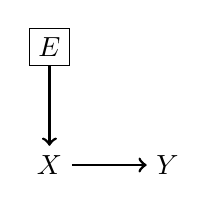
\begin{tikzpicture}
	     % nodes %
		 \node[text centered] (x) {$X$};
		 \node[right of = x, node distance=1.5cm, text centered] (y) {$Y$};
		 %\node[above of = y, node distance=1.5cm, text centered] (x) {$X$};
		 %\node[right of = y, above of=y, node distance=.75cm, text centered] (u) {$U$};
		 \node[draw, rectangle, above of = x, node distance=1.5cm, text centered] (e) {$E$};
		
		 % edges %
		 \draw[->, line width = 1] (x) --  (y);
		 \draw[->, line width = 1] (e) -- (x);
	     \end{tikzpicture}
	\caption{causal prediction}
	\label{fig:causal}
\end{figure}

\begin{figure}
  \centering
  \tikzsetnextfilename{anticausal1}
    \begin{tikzpicture}
    % nodes %
      \node[text centered] (x) {$X$};
      \node[right of = x, node distance=1.5cm, text centered] (y) {$Y$};
      %\node[above of = y, node distance=1.5cm, text centered] (x) {$X$};
      %\node[right of = y, above of=y, node distance=.75cm, text centered] (u) {$U$};
      \node[draw=none, above of = x, node distance=1.5cm, text centered] (e) {};

      % edges %
      \draw[->, line width = 1] (y) --  (x);
    \end{tikzpicture}
  \caption{anti-causal prediction}
  \label{fig:anticausal}
\end{figure}

\begin{figure}
  \centering
  \tikzsetnextfilename{anticausal}
    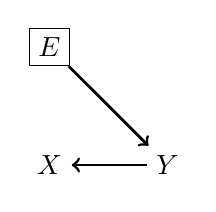
\begin{tikzpicture}
    % nodes %
      \node[text centered] (x) {$X$};
      \node[right of = x, node distance=1.5cm, text centered] (y) {$Y$};
      %\node[above of = y, node distance=1.5cm, text centered] (x) {$X$};
      %\node[right of = y, above of=y, node distance=.75cm, text centered] (u) {$U$};
      \node[draw, rectangle, above of = x, node distance=1.5cm, text centered] (e) {$E$};

      % edges %
      \draw[->, line width = 1] (y) --  (x);
      \draw[->, line width = 1] (e) -- (y);
    \end{tikzpicture}
  \caption{anti-causal prediction}
  \label{fig:anticausal}
\end{figure}

	\begin{figure}
	    \centering
	    \tikzsetnextfilename{confounded1}
	     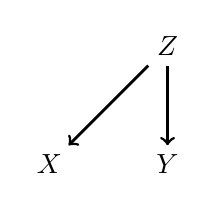
\begin{tikzpicture}
	     % nodes %
      \node[text centered] (x) {$X$};
      \node[right of = x, node distance=1.5cm, text centered] (y) {$Y$};
      \node[above of = y, node distance=1.5cm, text centered] (z) {$Z$};
      %\node[right of = y, above of=y, node distance=.75cm, text centered] (u) {$U$};
      \node[draw=none, above of = x, node distance=1.5cm, text centered] (e) {};

      % edges %
      \draw[->, line width = 1] (z) --  (x);
      \draw[->, line width = 1] (z) --  (y);
        \end{tikzpicture}
	\label{fig:fork}
\end{figure}


	\begin{figure}
	    \centering
	    \tikzsetnextfilename{confounded}
	     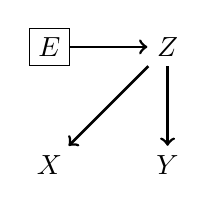
\begin{tikzpicture}
	     % nodes %
      \node[text centered] (x) {$X$};
      \node[right of = x, node distance=1.5cm, text centered] (y) {$Y$};
      \node[above of = y, node distance=1.5cm, text centered] (z) {$Z$};
      %\node[right of = y, above of=y, node distance=.75cm, text centered] (u) {$U$};
      \node[draw, rectangle, above of = x, node distance=1.5cm, text centered] (e) {$E$};

      % edges %
      \draw[->, line width = 1] (z) --  (x);
      \draw[->, line width = 1] (z) --  (y);
      \draw[->, line width = 1] (e) -- (z);
        \end{tikzpicture}
	\label{fig:fork}
\end{figure}



%  \begin{figure}[ht!]
% 	\begin{subfigure}[b]{0.3\textwidth}
%      \centering
% 	     \begin{tikzpicture}
% 	     % nodes %
% 		 \node[text centered] (x) {$X$};
% 		 \node[right of = x, node distance=1.5cm, text centered] (y) {$Y$};
% 		 %\node[above of = y, node distance=1.5cm, text centered] (x) {$X$};
% 		 %\node[right of = y, above of=y, node distance=.75cm, text centered] (u) {$U$};
% 		 \node[draw, rectangle, above of = x, node distance=1.5cm, text centered] (e) {$E$};
%
% 		 % edges %
% 		 \draw[->, line width = 1] (x) --  (y);
% 		 \draw[->, line width = 1] (e) -- (x);
% 	     \end{tikzpicture}
% 	\caption{causal prediction}
% 	\label{fig:causal}
% %\begin{align*}
%     %& p(X,Y|E) \\
%     %&= p(Y|X,E)p(X|E) \\
%     %&= p(Y|X)p(X|E)
% %\end{align*}
%      \end{subfigure}
% \hfill
% 	\begin{subfigure}[b]{0.3\textwidth}
%      \centering
% 	     \begin{tikzpicture}
% 	     % nodes %
% 		 \node[text centered] (x) {$X$};
% 		 \node[right of = x, node distance=1.5cm, text centered] (y) {$Y$};
% 		 %\node[above of = y, node distance=1.5cm, text centered] (x) {$X$};
% 		 %\node[right of = y, above of=y, node distance=.75cm, text centered] (u) {$U$};
% 		 \node[draw, rectangle, above of = x, node distance=1.5cm, text centered] (e) {$E$};
%
% 		 % edges %
% 		 \draw[->, line width = 1] (y) --  (x);
% 		 \draw[->, line width = 1] (e) -- (y);
% 	     \end{tikzpicture}
% 	\caption{anti-causal prediction}
% 	\label{fig:anticausal}
% %\begin{align*}
%     %& p(X,Y|E) \\
%     %&= p(X|Y,E)p(Y|E) \\
%     %&= p(X|Y)p(Y|E)
% %\end{align*}
%      \end{subfigure}
% \hfill
% 	\begin{subfigure}[b]{0.3\textwidth}
%      \centering
% 	     \begin{tikzpicture}
% 	     % nodes %
% 		 \node[text centered] (x) {$X$};
% 		 \node[right of = x, node distance=1.5cm, text centered] (y) {$Y$};
% 		 \node[above of = y, node distance=1.5cm, text centered] (z) {$Z$};
% 		 %\node[right of = y, above of=y, node distance=.75cm, text centered] (u) {$U$};
% 		 \node[draw, rectangle, above of = x, node distance=1.5cm, text centered] (e) {$E$};
%
% 		 % edges %
% 		 \draw[->, line width = 1] (z) --  (x);
% 		 \draw[->, line width = 1] (z) --  (y);
% 		 \draw[->, line width = 1] (e) -- (z);
% 	     \end{tikzpicture}
% 	\caption{confounded prediction}
% 	\label{fig:fork}
%      \end{subfigure}
%      \caption{directed acyclic graphs for 2-variable prediction problems with a shift in case-mix, meaning the environment variable only affects the marginal distribution of one variable but not a conditional distribution. The prediction is always made from $X$ to $Y$. $X$ denotes an arbitrary set of features with arbitrary feature types.}
%      \label{fig:dags}
%  \end{figure}

\end{document}
